\cotefile{37}
\scanpage{8}
\begin{flushright}
SGA 4
\end{flushright}
% archive sheet number: 7

\scanpage{14}
\begin{center}
\textsc{Brandeis University}\\
\textsc{Waltham, Massachusetts 02154}
\end{center}
\noindent DEPARTMENT OF MATHEMATICS\hfill le 28 Mai.\\

\margin{P.S. Je demanderai à Mike s'il veut s'occuper des exp. après VI.}
Cher Grothendieck,\\

Nous avions décidé de mettre l'appendice ``Image inverse d'un plat'' à l'exposé $\underline{\overline{\mathrm{V}}}$ et l'appendice ``Assez de points'' à l'exposé VI. Ils ne concernent donc pas l'exposé $\underline{\overline{\mathrm{IV}}}$.

Je vais t'envoyer une version non canulée de \makebox[0pt][l]{\tikz[overlay,baseline=0pt]{\draw[gray,thin,rotate around={10:(1.5em,.3em)}] (3.38em,.59em) arc[start angle=20,end angle=345,x radius=2em,y radius=.85em]; \draw[gray!60,thin,rotate around={10:(1.5em,.3em)}] (.60em,-.52em) .. controls (1.95em,-.70em) and (3.13em,-.19em) .. (3.46em,.35em);}}4.10.6.

Peux tu me faire envoyer une copie de $\underline{\overline{\mathrm{IV}}}$ \S\,9-13 ?

Je passe quelques jours à Paris pour le : \deleted{Congrès} Séminaire \unsure{Bourbaki|Boubaki}, Mais tu n'y viendra probablement pas.

J'ai beaucoup aimé ton article avec Godement.

\begin{flushright}
Bien cordialement\\
\unsure{Johny|Johnny}\\
\end{flushright}
% archive sheet number: 13

\scanpage{17}
\begin{center}
INSTITUT\\
DES HAUTES ÉTUDES SCIENTIFIQUES\\
\rule{2.3em}{0.4pt}
\end{center}

\uline{Continuation de} SGA 4 $\underline{\overline{\mathrm{IV}}}$ 4.10.6 (\makebox[0pt][l]{\tikz[overlay,baseline=0pt,x=1em,y=1em]{\draw[gray,thin] (-.45,-1.1) .. controls (-.55,-.25) and (.1,-.35) .. (1.3,-.35) -- (8.1,-.35) .. controls (8.9,-.35) and (9.1,-.1) .. (9,.55);}}\inserted{généralisation des} 3° et 4°\unsure{)} appliqué à $S(x)\subset S_{/x}$)

5°) Soit $S_0\hookrightarrow S$ une \deleted{\unsure{foncteur|foncteurs} ($S_0$ cat. \unsure{$\in\mathcal{U}$|$\subset\mathcal{U}$|$\mathcal{U}$}) et supposons que} sous-catégorie pleine de $S$ satisfaisant les conditions suivantes :

(i) Si $u:X\mathbin{-}Y$ avec $u\in\underline{M}$, $Y\in\mathrm{ob}\,S_0$, donc $X\in\mathrm{ob}\,S_0$

[ (ii) \deleted{$\forall X\in\mathrm{ob}\,S$, existe famille \unsure{couvrante|couvrant} $X_i\to X$, \unsure{telle} \unsure{que $X_i$|$Y_i\mathbin{-}X_i$} \unsure{tq|soit}} le crible de $S$ engendré par les objets de $S_0$ est couvrant, i.e. $\forall X\in\mathrm{ob}\,S$, existe famille couvrante $X_i\to X$, avec $X_i\to Z_i\in\mathrm{ob}\,S_0$. ]

\unsure{.} Munissons $S_0$ de la top. induite. \unsure{Prouver|Prouvons} qu'une famille de morphismes $X_i-X$ dans $S_0$ est couvrante dans $S_0$ ssi elle l'est dans $S_{\deleted{\unsure{0}}}$ et que $S_0\to S$ est \uline{cocontinu.}

Soit $\underline{M}_0$ l'ens des $u\in\underline{M}$, \deleted{\unsure{tq}} $u:x-y$, avec $Y\in\mathrm{ob}\,S_0$, donc $X\in\mathrm{ob}\,S_0$. \unsure{Prouver|Prouvons} que $\underline{M}_0\in\mathrm{Fl}(S_0)$ satisfait les conditions a) b) c) d) de \uline{1}°).

Procédant comme dans 3°, définir des foncteurs
\par\noindent
\begin{tabular}{@{}l@{\quad}l@{}}
$\mathrm{Res}:\widetilde{S}\to\widetilde{S}_0,$ & \makebox[0pt][l]{\tikz[overlay,baseline=0pt,x=1em,y=1em]{\draw[gray,thin] (9.4,1.35) .. controls (10,2.1) and (-.9,1.7) .. (-.8,.35) .. controls (-1,-2.3) and (8.8,-2.3) .. (10,-.65) .. controls (10.5,.15) and (10.1,.8) .. (9.8,1.05);}}$\mathrm{Prol}:\widetilde{S}_0\mathbin{-}\widetilde{S}_{\deleted{\unsure{0|2}}}\;?$\\
\deleted{et \unsure{prouver|prouvons} que}\inserted{tels que} $\mathrm{Res}$ comm. & aux limites
\end{tabular}\par\noindent
inductives et projectives, et $\mathrm{Prol}$ est exact \unsure{à|:} g. et pl fidèle, son image essentielle
% archive sheet number: 16

\scanpage{19}
SGA 4 $\underline{\overline{\mathrm{XVII}}}$

\diagram{\(\begin{array}{@{}l l l@{}}
\text{p.75} & \text{l.}\,-4 & \text{réf \deleted{\unsure{à|q|?}} à } \underline{\overline{\mathrm{V}}}\ \text{\unsure{correcte|corrects} ?}\\
\text{p.90} & \text{l.}\ 2 & \text{ref : } f_!\ \text{pour Ensembles pointés resp. faisceaux}\\
&&\hfill\text{en \unsure{Groupes|groupes} ??}\\
&&\text{\unsure{Consulter|(consulter} Verdier)}\\[3pt]
\text{p.139} & \text{l.}\,-10 & \text{ref : }\underline{\overline{\mathrm{VI}}}_{\mathrm B}\\
\text{p.167} & \text{l.}\,-8 & \text{réf : EGA }\underline{\overline{\mathrm{II}}}\ \unsure{2^{\mathrm e}|?^{\mathrm e}}\ \text{édition (lemme de Chow)}\\
170 & \text{l.}\ 7 & \smash{\raisebox{-.55\baselineskip}{\(\left\{\vphantom{\begin{array}{c}0\\0\end{array}}\right.\)}}\ \text{réf : }\underline{\overline{\mathrm V}}\ \text{- \unsure{W.|v.} Deligne .--}\\
175 & \text{l.}\,-1 & \phantom{\{}\ \text{id}
\end{array}\)}
% archive sheet number: 18

\scanpage{20}
\uline{SGA 4}\qquad F\uline{asc.} 1
\margin{\(\left\{\ \text{\uline{Topologie générale}}\right.\)}

\diagram{\(\begin{array}[t]{@{}l@{\quad}l@{}}
\left\{\begin{array}[t]{l}
\text{\unsure{Preface|Préface}, avant-propos,}\smash{\rlap{\tikz[overlay]{\draw[thin] (0,-.2ex) .. controls (2em,-.4ex) and (1.5em,-9.4ex) .. (3em,-13.8ex) .. controls (5em,-14.5ex) and (12em,-16ex) .. (15em,-14.5ex);}}}\\
\text{Exp I \unsure{à|:} }\underline{\overline{\mathrm{IV}}}
\end{array}\right. &
\begin{array}[t]{l}
\text{table des matières}\\
\text{générale du Sém.}\\
\text{Table des matières}\\
\text{du Volume.}\\
\text{index \unsure{alphabétique}.}\\
\#\,570\ \text{p.}
\end{array}
\end{array}\)}

F\uline{asc}. 2\qquad Exp. \(\begin{array}[t]{@{}cccccccc@{}}\underline{\overline{\mathrm{V}}}&\underline{\overline{\mathrm{VI}}}&\smash{\rlap{\tikz[overlay,baseline=0pt,x=1em,y=1ex]{\draw[thin] (0,.65) .. controls (.05,-.4) and (-1.65,-1.7) .. (-1.65,-3.2); \draw[thin] (0,.65) .. controls (-.1,-.55) and (1.55,-1.3) .. (1.65,-3.15);}}}&\underline{\overline{\mathrm{VII}}}&\underline{\overline{\mathrm{VIII}}},&\underline{\overline{\mathrm{IX}}}&\underline{\overline{\mathrm{X}}}&\underline{\overline{\mathrm{XI}}}\\[1.1ex]&&\inserted{\underline{\overline{\mathrm{VI}}}_{\mathrm B}}&&&&&\end{array}\)
\margin{\(\left\{\begin{array}{l}\text{\uline{Cohomologie des}}\\\text{\uline{topos et les}}\\\text{\uline{sites étales} :}\\\text{\uline{étude générale}}\end{array}\right.\)}

F\uline{asc}. 3
\margin{Théorèmes de \unsure{ch\textsuperscript{t}|ch\textsuperscript{gt}} de base et de dualité globale}

\diagram{\(\begin{array}{@{}l r l@{}}
 \underline{\overline{\mathrm{V}}} &100&\\
 \underline{\overline{\mathrm{VI}}}&150&\\
 \underline{\overline{\mathrm{VI}}}_{\mathrm B}&30&\\
 \cline{1-2}
 &\deleted{\unsure{11|40}}&\smash{\rlap{\tikz[overlay]{\draw[thin] (-1em,.9ex) .. controls (0,-1ex) and (1.8em,-3ex) .. (2.8em,-8ex) .. controls (3.6em,-12ex) and (4em,-19ex) .. (6em,-19ex); \draw[thin] (3.4em,.2ex) .. controls (3.4em,-.8ex) and (4.2em,-1.2ex) .. (4em,-2.1ex) .. controls (3.7em,-2.5ex) and (4.25em,-2.7ex) .. (4.4em,-3.1ex) .. controls (4.65em,-3.7ex) and (4.55em,-4.9ex) .. (5.4em,-5.7ex);}}}\text{\deleted{\uline{Cat. Dérivées} \unsure{42|40}}}\\
 \underline{\overline{\mathrm{VII}}}&24&\\
 \underline{\overline{\mathrm{VIII}}}&46&\\ \cline{2-2}
 \underline{\overline{\mathrm{IX}}}&\deleted{\unsure{330|630|530}}&\\
 &42&\\
 \mathrm X&21&\\
 \mathrm{XI}&19&\deleted{\unsure{\mathrm{Cat.}}}\quad
 \text{\makebox[0pt][l]{\tikz[overlay,baseline=0pt]{\draw[thin,rotate around={8:(3.7em,.3em)}] (2.435em,1.052em) arc[start angle=110,end angle=455,x radius=3.7em,y radius=.8em]; \draw[thin] (-4em,-.5ex) .. controls (-1.4em,-1ex) and (-.2em,.7ex) .. (1.4em,1.6ex);}}Cat. dér. ? 40}\\
 \cline{2-2}\cline{2-2}
 &432&\\ \hline
\end{array}\)}

\diagram{\(\begin{array}{@{}l l@{}}
\left.\begin{array}{@{}l r@{}}
\underline{\overline{\mathrm{XII}}}&57\\\underline{\overline{\mathrm{XIII}}}&15\\\underline{\overline{\mathrm{XIV}}}&\unsure{24|74}\\
\underline{\overline{\mathrm{XV}}}&38\\\underline{\overline{\mathrm{XVI}}}&44
\end{array}\right\} & \raisebox{-2.6ex}{\(\cdot\ 178\)}\\
\begin{array}{@{}l r@{}}
\underline{\overline{\mathrm{XVII}}}&210\\\underline{\overline{\mathrm{XVIII}}}&200\\\underline{\overline{\mathrm{XI}}\mathrm{X}}^{\unsure{\prime}}&51\\\cline{2-2}
&\#\,640
\end{array} & \raisebox{2.5ex}{\(\unsure{5|\int}\)}
\end{array}\)}
% archive sheet number: 19

\scanpage{21}
\begingroup
\setbox0=\vbox{\hsize=\linewidth
\noindent\uline{Il faut} \deleted{\illegible{2}} \uline{\unsure{insérez|insérer} le texte manquant en une} \unsure{pge|page} 83 bis, dans laquelle il faudra reporter le texte des lignes 7 à 18 du \deleted{\unsure{blanc}}\inserted{stencil} 84\par
\medskip
\noindent me montrer la frappe \deleted{faite}\par
\diagram{\(\begin{array}{@{}l l l@{}}
\text{p.85} &\text{l.13} &\mathbb Lg^{\ast}\quad \mathbb Lg'^{\ast}\\
&\text{l.23} &\mathbb Lg^{\unsure{+|\ast}}\quad\mathbb Lg^{\unsure{\ast|+}}\\
&\text{l.39} &\mathbb Lg'^{\ast}\\
&\text{l.27 et suite :} &\text{\uline{Le texte oublié a été reporté ici}}\\
&&\text{\uline{par erreur} !!!}
\end{array}\)}
}
\edef\cancelwidth{\the\wd0}
\edef\cancelheight{\the\dimexpr\ht0+\dp0\relax}
\noindent\hbox{\copy0%
\begin{tikzpicture}[overlay,x=\cancelwidth,y=\cancelheight]
\draw[black!55,line width=.45pt] (-.60,.95) -- (-.89,.11);
\draw[black!55,line width=.45pt] (-.20,1.00) -- (-.57,.01);
\draw[black!55,line width=.45pt] (-.02,.82) -- (-.32,.03);
\end{tikzpicture}}
\endgroup
\par

\diagram{\(\begin{array}{r@{\qquad}l}
210&\\
\deleted{\unsure{4|2}}76&\\
250&\text{Fasc.}\\
\makebox[0pt][l]{\tikz[baseline=0pt,overlay,x=1em,y=1em]{\draw[thin] (-.7,.65) -- (2.2,1.25); \begin{scope}[shift={(.7,-.1)},rotate=32]\draw[thin] (0,0) ellipse (1.8 and .85);\end{scope}}}536&
\end{array}\)}
% archive sheet number: 20

\scanpage{22}
\begin{center}
INSTITUT\\
DES HAUTES ÉTUDES SCIENTIFIQUES\\
\rule{2.3em}{0.4pt}
\end{center}
SGA 4 $\underline{\overline{\mathrm{VI}}}$

Introduction : signaler \unsure{produits} ``sans doute lié au fait que tout end. d'un \unsure{point} est un autom.''\unsure{)|\}}

\S\,4\qquad Changer \(E_{/\varphi}\) en \({}_{\varphi}\backslash E\)

\S\,3 (?)\qquad Changer l'exercice sur les topos finis.

\S\,4\qquad Supprimer réf au cas noeth (traité mieux dans l'exercice de $\underline{\overline{\mathrm{IV}}}$ 9.1 ?

\S\,1\qquad 1.25,\textemdash\,- vérifier si c'est correct. Remplacer ``$\exists$ sommes \deleted{\unsure{amalgamées}}\inserted{\unsure{en deux obj|de deux obj}} et \unsure{initial|initiale|toutes|totales}'' \deleted{\unsure{si|et}} par ``$\exists$ $\unsure{\underrightarrow{\mathrm{lim}}|\underline{\mathrm{lim}}}$ finies''

\S\ ,\qquad \unsure{Exercice|Éxercice} : $\underrightarrow{\mathrm{Limtop}}$ (\unsure{commuter|commute} trivialement\unsure{?})
% archive sheet number: 21

\scanpage{26}
\deleted{\unsure{E}}\unsure{S|E}GA 4 $\underline{\overline{\mathrm{IV}}}$
\diagram{\(\left\{\begin{array}{l}
\text{Modules plats sur anneau non commutatif \unsure{:|,} \unsure{mot|mt} ?}\\
\unsure{f|J}_!\ \text{pour Ensembles pointés ou Groupes (pas réf \unsure{/|y} aucun)}
\end{array}\right.\)}

SGA 4 $\underline{\overline{\mathrm{XVII}}}$ 4.23 attention réf à $\underline{\overline{\mathrm{V}}}$ \unsure{3|1}.7 (changée ?)

$\underline{\overline{\mathrm{XVII}}}$\qquad Théorème de finitude pour faisceau d'anneaux de torsion quelconque.

Préface à 2\textsuperscript{ème} édition. Signaler autres contributions de Deligne
\diagram{\(\left|\begin{array}{l}
\text{b) Intégration des torseurs}\\
\text{a) Trace des torseurs}\\
\text{\hspace{1em}sous conditions inhabituelles}
\end{array}\right.\)}

\noindent\rule{\linewidth}{0.4pt}

Que faire avec C.D. de Verdier : inclure ?

\noindent\rule{\linewidth}{0.4pt}

SGA 4 $\underline{\overline{\mathrm{IV}}}$\qquad Exercices \unsure{à|:} \unsure{reporter|rajouter} : \S\,8
\diagram{\(\left|\begin{array}{l}
\text{topos locaux}\\
\text{topos pseudoponctuels}\\
\text{topos }I^{\wedge}, I\ \text{\unsure{ens|un} ordonné,}
\end{array}\right.\)}
% archive sheet number: 25

\scanpage{28}
SGA 4 $\underline{\overline{\mathrm{XVI}}}$ 1\qquad \unsure{compléter|Compléter} comme dans Giraud
% archive sheet number: 27

\scanpage{33}
\noindent\begin{tabular}{@{}l|l@{}}
I\uline{ntroduction} vider & Bibliographie mixte.\\
 & mention de C.T.
\end{tabular}

\begin{center}
INSTITUT\\
DES HAUTES ÉTUDES SCIENTIFIQUES\\
\rule{2.3em}{0.4pt}
\end{center}

\uline{Artin}\qquad SGA 4

réf \quad X \quad [1]

X \qquad p.7 \qquad Début de phrase manque

\noindent\rule{\linewidth}{0.4pt}

$\underline{\overline{\mathrm{X}}\mathrm{I}\overline{\mathrm{I}}}$\qquad compléter réf : Giraud

5.10. \qquad \unsure{Compléter|compléter} remarque par réf.\\
\hspace*{5em}aux travaux récents d'Artin

{\color{red!75!black}
\noindent
\begin{tikzpicture}[x=\linewidth,y=1ex,baseline=0pt]
\draw[line width=.4pt] (0,0) .. controls (.07,.8) and (.12,1) .. (.17,.55)
 .. controls (.25,.1) and (.29,-.2) .. (.32,.15);
\end{tikzpicture}

$\underline{\overline{\mathrm{IX}}}$\qquad p\unsure{.}\,34 \qquad \unsure{réf|ref} th. de Tsen
}

\noindent\rule{.6\linewidth}{0.4pt}

$\underline{\overline{\mathrm{XIII}}}$\qquad \deleted{p.\unsure{13}} 3.1. \qquad Supposer $X$ noethérien\\
\hspace*{7em}(sinon, p.13 l.$-3$ pas clair)

{\color{gray!80!black}
\noindent\rule{.42\linewidth}{0.4pt}

XIX \qquad p 3,4,10 \qquad p 7 \deleted{\unsure{14|24}},\unsure{18|10},55,39,43
}
% archive sheet number: 32

\scanpage{36}

\begingroup
\dimen0=\linewidth
\dimen2=\dimen0
\divide\dimen2 by 990
\edef\scanunit{\the\dimen2}
\dimen4=1000\dimen2
\setbox0=\vbox to\dimen4{%
  \offinterlineskip
  \hsize=\linewidth
  \kern80\dimen2
  \setbox2=\hbox to\linewidth{%
    \kern120\dimen2\rlap{Exposés}%
    \kern190\dimen2\rlap{$\underline{\overline{\mathrm{XI}}}$}%
    \kern98\dimen2\rlap{à}%
    \kern72\dimen2\rlap{$\underline{\overline{\mathrm{XIV}}}$}%
    \kern122\dimen2\rlap{sont}%
    \kern125\dimen2\rlap{tapés}\hfil}%
  \ht2=0pt\dp2=0pt\box2
  \kern89\dimen2
  \setbox2=\hbox to\linewidth{%
    \kern150\dimen2\rlap{avec}%
    \kern198\dimen2\rlap{des}%
    \kern91\dimen2\rlap{caractères}%
    \kern250\dimen2\rlap{plus}%
    \kern109\dimen2\rlap{gros}\hfil}%
  \ht2=0pt\dp2=0pt\box2
  \kern72\dimen2
  \setbox2=\hbox to\linewidth{%
    \kern188\dimen2\rlap{que}%
    \kern122\dimen2\rlap{le}%
    \kern96\dimen2\rlap{reste}%
    \kern129\dimen2\rlap{du}%
    \kern85\dimen2\rlap{Séminaire.}\hfil}%
  \ht2=0pt\dp2=0pt\box2
  \kern174\dimen2
  \setbox2=\hbox to\linewidth{%
    \kern147\dimen2\rlap{Vider}%
    \kern153\dimen2\rlap{sommaires}%
    \kern298\dimen2\rlap{\raise12\dimen2\hbox{(des}}%
    \kern106\dimen2\rlap{\raise15\dimen2\hbox{exposés}}%
    \kern166\dimen2\rlap{\raise20\dimen2\hbox{$\underline{\overline{\mathrm{XVI}}}$,}}\hfil}%
  \ht2=0pt\dp2=0pt\box2
  \kern55\dimen2
  \setbox2=\hbox to\linewidth{%
    \kern755\dimen2
    \unsure{$\underline{\overline{\mathrm{XIV}}}$|$\underline{\overline{\mathrm{XIX}}}$}\ .\,.\,--)\ ?\hfil}%
  \ht2=0pt\dp2=0pt\box2
  \kern210\dimen2
  \setbox2=\hbox to\linewidth{%
    \kern110\dimen2\rlap{$\underline{\overline{\mathrm{VI}}}$}%
    \kern138\dimen2\rlap{p.49,}%
    \kern132\dimen2\rlap{\raise16\dimen2\hbox{p.50}}%
    \kern192\dimen2\rlap{\raise43\dimen2\hbox{\unsure{univers}}}%
    \kern148\dimen2\rlap{\raise58\dimen2\hbox{est}}%
    \kern75\dimen2\rlap{\raise65\dimen2\hbox{\uline{non vide}\ !}}\hfil}%
  \ht2=0pt\dp2=0pt\box2
  \kern45\dimen2
  \setbox2=\hbox to\linewidth{%
    \kern377\dimen2\rlap{p.52}%
    \kern163\dimen2\rlap{\raise20\dimen2\hbox{vider}}%
    \kern148\dimen2\rlap{\raise38\dimen2\hbox{footnote}}\hfil}%
  \ht2=0pt\dp2=0pt\box2
  \kern185\dimen2
  \setbox2=\hbox to\linewidth{%
    \kern116\dimen2\rlap{$\underline{\overline{\mathrm{VIII}}}$}%
    \kern178\dimen2\rlap{généralités}%
    \kern226\dimen2\rlap{\raise18\dimen2\hbox{sur}}%
    \kern99\dimen2\rlap{\raise21\dimen2\hbox{foncteurs}}%
    \kern215\dimen2\rlap{\raise30\dimen2\hbox{\unsure{fibre|fibres} :}}\hfil}%
  \ht2=0pt\dp2=0pt\box2
  \kern55\dimen2
  \setbox2=\hbox to\linewidth{%
    \kern294\dimen2\rlap{renvoyer à}%
    \kern265\dimen2\deleted{\unsure{SG|SGA}}\quad
    $\underline{\overline{\mathrm{IV}}}$\ \ldots--\hfil}%
  \ht2=0pt\dp2=0pt\box2
  \vss
}%
\noindent\hbox{%
  \rlap{\raise\ht0\hbox{%
    \begin{tikzpicture}[overlay,baseline=0pt,x=\scanunit,y=-\scanunit,line cap=round,line join=round]
      \begin{scope}[shift={(-80,-90)}]
        \draw[black!75,line width=.3pt] (80,418) -- (1017,398);
        \draw[black!75,line width=.3pt] (95,684) -- (1037,613);
        \draw[black!50,line width=.7pt] (120,415) .. controls (245,280) and (388,91) .. (408,94);
        \draw[black!50,line width=.7pt] (365,415) .. controls (511,273) and (671,72) .. (690,95);
        \draw[black!50,line width=.7pt] (626,427) .. controls (745,299) and (870,188) .. (936,160);
        \draw[black!50,line width=.55pt] (874,433) .. controls (899,368) and (934,340) .. (947,330);
        \draw[black!55,line width=.7pt]
          (260,461) .. controls (220,526) and (87,818) .. (94,838)
          .. controls (104,886) and (359,450) .. (385,446)
          .. controls (410,422) and (245,801) .. (255,826)
          .. controls (269,858) and (549,420) .. (574,418)
          .. controls (611,398) and (384,834) .. (400,848)
          .. controls (417,880) and (736,458) .. (762,453)
          .. controls (806,429) and (588,855) .. (603,898)
          .. controls (607,953) and (650,941) .. (674,931);
        \draw[black!28,line width=.65pt]
          (308,449) .. controls (371,408) and (231,627) .. (229,643)
          .. controls (246,671) and (497,435) .. (520,427)
          .. controls (562,408) and (394,603) .. (406,615)
          .. controls (427,648) and (699,427) .. (721,420)
          .. controls (764,400) and (627,574) .. (642,585)
          .. controls (659,614) and (895,432) .. (925,423)
          .. controls (961,411) and (813,579) .. (832,590)
          .. controls (851,608) and (978,537) .. (1010,530);
        \draw[black!35,line width=.65pt]
          (202,706) .. controls (186,721) and (134,799) .. (139,810)
          .. controls (159,817) and (295,682) .. (311,681)
          .. controls (341,671) and (207,843) .. (217,859)
          .. controls (238,880) and (459,698) .. (483,690)
          .. controls (522,673) and (389,848) .. (402,863)
          .. controls (424,886) and (692,680) .. (716,674)
          .. controls (755,663) and (593,845) .. (604,856)
          .. controls (624,878) and (907,637) .. (934,630)
          .. controls (977,617) and (770,826) .. (784,836)
          .. controls (808,850) and (961,710) .. (980,709)
          .. controls (997,705) and (983,731) .. (984,739);
      \end{scope}
    \end{tikzpicture}%
  }}%
  \box0
}\par
\endgroup

% archive sheet number: 35

\scanpage{37}
\begin{flushright}
\rotatebox{180}{\sffamily\begin{tabular}{c}
INSTITUT\\
DES HAUTES ETUDES SCIENTIFIQUES\\
\rule{2em}{0.4pt}
\end{tabular}}
\end{flushright}
% archive sheet number: 36

\scanpage{38}
\begin{center}
INSTITUT\\
DES HAUTES ÉTUDES SCIENTIFIQUES\\
\rule{2.3em}{0.4pt}
\end{center}

\noindent\begin{minipage}{0.6\linewidth}
SGA 4 $\underline{\overline{\mathrm{XVIII}}}$\\[0.8em]
\hspace*{3em}\rlap{\begin{tikzpicture}[overlay,x=1em,y=1em]
\draw[line width=.35pt] (1.0,-.6) .. controls (-1.0,-.5) and (-.8,.7) .. (1.0,.9)
 .. controls (3.1,1.1) and (7.1,1.2) .. (7.8,2.7);
\end{tikzpicture}}\inserted{(Deligne)}
\end{minipage}

\medskip
\noindent Références pour SGA 5 $\underline{\overline{\mathrm{VII}}}$\quad
$\left\{\begin{array}{@{}l@{}}
\text{Dém de 3.\deleted{\unsure{6}}5.3.}\\[.4em]
\text{1.1\qquad b)}
\end{array}\right.$

\medskip
\noindent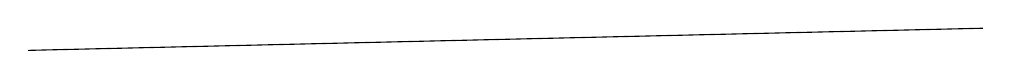
\begin{tikzpicture}[x=\linewidth,y=1em]
\draw[line width=.4pt] (0,0)--(1,.8);
\end{tikzpicture}

$\underline{\overline{\mathrm{V}}}$\qquad dire quelques mots sur relations\\
\hspace*{2.7em}avec $\underleftarrow{\mathrm{lim}}$ et ${\underleftarrow{\mathrm{lim}}}^{(p)}$ :

a) Sur un topos de \unsure{la} forme $\widehat C$,\\
\hspace*{1.4em}les foncteurs $H^n$ sont les $\mathop{\underleftarrow{\mathrm{lim}}}\nolimits_C^{(n)}$

b) Je \unsure{n'ai|n'y a} plus une telle interpré-\\
\hspace*{1.4em}tation pour un topos général,\\
\hspace*{1.4em}puisqu'on est obligé de prendre
\margin{\raisebox{-3.5em}[0pt][0pt]{\rule{.35pt}{5.5em}}\hspace{.35em}\begin{tabular}[t]{@{}l@{}}si ça\\marche \ldots\end{tabular}}
\[
 H^{n}(\deleted{\unsure{E|C}}\unsure{\widetilde C|\widetilde E},F)\simeq
 \mathop{\underrightarrow{\mathrm{lim}}}_{\mathcal U\in\mathcal R}
 \mathop{\underleftarrow{\mathrm{lim}}}_{\mathcal U}
 \deleted{\unsure{H^n|F^n}}\unsure{F^{n}/\mathcal U_{\varphi}|F/\mathcal U_{\varphi}|F/C_{/\varphi}}
\]

$\mathcal U$ crible variable

On a un recouvrement de l'objet final de $\widehat C$ par les objets de $C$

\bigskip
\noindent\hspace*{2.4em}$X\unsure{\times|+}Y$
% archive sheet number: 37

\cotefile{37}
\scanpage{47}

\diagram{\begin{tikzcd}[ampersand replacement=\&,column sep=large]
 E' \arrow[r,shift right=.55ex,"\varphi'"'] \&
 E'' \arrow[l,shift right=.55ex,"\varphi''"']
\end{tikzcd}
\quad
\begingroup
\setbox0=\hbox{$\left\{\begin{aligned}
\deleted{\lambda'\colon\operatorname{id}_{E'}\longrightarrow\unsure{\varphi'|\varphi}\varphi''}\\
\deleted{\lambda''\colon\operatorname{id}_{E''}\longrightarrow\varphi''\unsure{\varphi'|\varphi}}
\end{aligned}\right.$}
\dimen0=\dimexpr\ht0+\dp0\relax
\makebox[0pt][l]{\begin{tikzpicture}[overlay,x=\wd0,y=\dimen0]
\draw[thin] (.02,-.02)
 .. controls (.25,.70) and (.34,.54) .. (.24,-.34)
 .. controls (.55,.43) and (.70,.72) .. (.55,-.29)
 .. controls (.87,.31) and (.98,.78) .. (.86,-.14)
 .. controls (1.01,.11) and (1.03,.37) .. (.96,-.27)
 .. controls (.96,-.43) and (1.02,-.36) .. (1.05,-.30);
\end{tikzpicture}}%
\box0
\endgroup}

\diagram{\resizebox{\linewidth}{!}{\begin{tikzpicture}[x=.013cm,y=-.013cm,font=\footnotesize]
\node at (235,30) {\deleted{Esp fin}};
\node at (730,20) {\deleted{ord fin}};
\node at (242,190) {\deleted{\unsure{Espaces|Espace} \unsure{topologiques|top. quelconques|top. généraux} finis}};
\node at (850,165) {\deleted{ens préordonnés finis}};
\node at (280,308) {\deleted{espaces sobres finis}};
\node at (880,285) {\deleted{ens ordonnés finis}};
\node at (323,438) {\deleted{\unsure{ens. ordonné fini modulaire|ens. ordonnés finis modulaires|ens. ordonnés finis ou dual}}};
\draw[<->] (400,28) -- (625,28);
\draw[<->] (230,65) -- (235,137);
\node at (337,106) {\deleted{topologie opposée}};
\draw (756,50) .. controls (750,65) and (758,101) .. (760,120)
 .. controls (762,132) and (751,132) .. (750,124);
\draw (756,50) -- (765,55);
\node at (888,84) {\deleted{ordre opposé}};
\draw[<->] (527,165) -- (597,165);
\node at (593,126) {$\deleted{X\mapsto X\ \text{avec rel. spéc}}$};
\node[align=center] at (490,216) {\deleted{topologie}\\\deleted{des cribles}};
\node at (578,203) {$\deleted{\mathrel{\reflectbox{$\mapsto$}}X}$};
\draw[->] (227,235) .. controls (228,254) and (231,264) .. (235,270);
\draw[->] (808,210) .. controls (808,242) and (815,262) .. (823,265);
\draw[->] (615,294) -- (537,294);
\draw[<->] (239,340) -- (239,405);
\draw[thin] (226,-75) -- (60,352) -- (68,345);
\draw[thin] (390,-28) -- (191,466) -- (204,450);
\draw[thin] (547,25) -- (347,492) -- (357,484);
\draw[thin] (769,45) -- (590,435) -- (600,427);
\draw[thin] (952,96) -- (804,351) -- (810,347);
\draw[thin] (1036,175) .. controls (1029,207) and (987,272) .. (982,285);
\end{tikzpicture}}}

\diagram{\resizebox{\linewidth}{!}{\begin{tikzpicture}[x=.013cm,y=-.013cm,font=\footnotesize]
\node at (125,45) {$\widehat{\mathrm E}$sp fin};
\node at (546,32) {préord fin};
\node at (170,160) {$X=(\mathscr X,T)\in\widehat{\mathrm E}\text{sp fin \unsure{sob|sb}}$};
\node at (665,125) {$\text{ord fin}\ni(\mathscr X,\omega)=I$};
\node at (471,266) {$\text{Lat fin mod }\sigma$};
\node at (510,386) {Top fin spec};
\draw[<->] (240,50) -- (451,40);
\draw[->] (145,84) .. controls (149,101) and (162,113) .. (178,122);
\draw[->] (514,64) .. controls (522,91) and (527,100) .. (537,100);
\draw[<->] (323,152) -- (506,139);
\draw[<->] (235,194) -- (338,275);
\node at (351,188) {$X\to\operatorname{Ouv}(X)$};
\node at (359,211) {\deleted{\unsure{ens des ouverts|ens des ouverts.|ens. des ouverts}}};
\draw[<->] (594,154) -- (546,236);
\node at (645,198) {ens des cri};
\draw[->] (438,347) .. controls (424,332) and (424,304) .. (439,295);
\draw[line width=.6pt] (438,347) -- (445,352) -- (442,343);
\draw[->] (468,296) -- (480,365);
\node at (375,316) {$E\mapsto\operatorname{Ouv}(E)$};
\node at (560,316) {$\sigma\to\sigma^\sim$};
\draw[->,thin] (503,340) .. controls (539,350) and (592,336) .. (612,335);
\node at (674,338) {top can};
\draw[->] (187,194) .. controls (175,315) and (322,332) .. (388,367);
\node at (202,337) {$\operatorname{Top}(X,T)$};
\draw[->,thin] (293,427) .. controls (65,430) and (76,314) .. (102,234);
\node at (77,375) {$E\to\operatorname{Point}(E)$};
\draw[->] (764,157) .. controls (870,283) and (770,350) .. (681,391);
\node at (873,280) {$(X,\omega)^\wedge$};
\draw[->,thin] (733,398) .. controls (1094,370) and (1010,247) .. (860,164);
\node at (1088,302) {$\unsure{\underline{\underline E}|\underline E|E}\to\text{\uline{Point}}(E)$};
\node at (1080,47) {$\deleted{\unsure{y\leftarrow x|y\to x}}$};
\draw[line width=.9pt] (1097,11) .. controls (1092,24) and (1074,30) .. (1059,29);
\draw[line width=.9pt] (1059,29) -- (1069,35);
\draw[line width=1.2pt] (1097,11) -- (1088,4);
\draw[line width=.7pt] (1097,11) -- (1102,3);
\node at (953,115) {$x\longleftarrow y$};
\node at (897,159) {\unsure{spé.|spéc.}};
\node at (1000,159) {gén};
\end{tikzpicture}}}

\begin{flushright}
\begin{minipage}{.56\linewidth}
\deleted{\unsure{ensemble polye.|ensemble polyéd.|ensemble polyèdre}}\quad
schéma simplicial
\makebox[0pt][l]{\raisebox{1.7ex}{\inserted{fini}}}%
\makebox[0pt][l]{\tikz[overlay,x=1em,y=1ex]{\draw[thin] (-.05,1.0)
 .. controls (.05,1.5) and (.7,1.5) .. (1.4,1.5)
 .. controls (2.3,1.6) and (2.8,2.0) .. (2.65,2.9);}}%
\unsure{(}$=$ ens avec\\
\deleted{\unsure{anti|enti|ensemble}}\ \unsure{filtre des|filtres des|filtre de|filtres de} parties.

$\deleted{x\leq y\qquad x\longrightarrow y}$
\end{minipage}
\end{flushright}

\noindent\begin{minipage}[t]{.72\linewidth}
\vspace{0pt}
\diagram{\resizebox{\linewidth}{!}{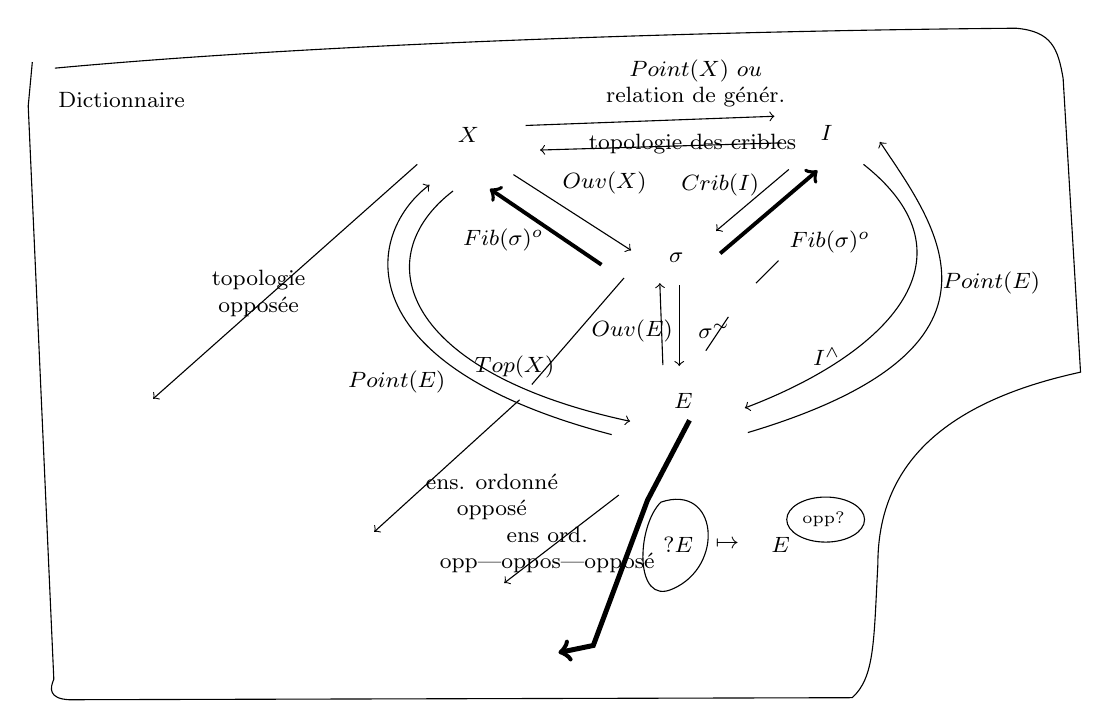
\begin{tikzpicture}[x=.013cm,y=-.013cm,font=\footnotesize]
\draw (26,45) .. controls (307,19) and (713,8) .. (965,6)
 .. controls (1000,9) and (1006,26) .. (1011,55)
 -- (1028,342)
 .. controls (876,375) and (830,447) .. (830,530)
 .. controls (826,605) and (827,640) .. (805,660)
 -- (40,662)
 .. controls (20,661) and (21,651) .. (25,642)
 -- (0,82) -- (4,39);
\node[anchor=west] at (20,76) {\uline{Dictionnaire}};
\node at (430,110) {$X$};
\node at (780,108) {$I$};
\node at (633,230) {$\sigma$};
\node at (640,370) {$E$};
\draw[->] (486,101) -- (729,92);
\draw[->] (736,118) -- (500,125);
\node[align=center] at (652,60) {$\text{\uline{Point}}(X)\ \text{ou}$\\relation de génér.};
\node at (649,119) {topologie des cribles};
\draw[->] (474,149) -- (589,223);
\draw[->,line width=1.4pt] (560,237) -- (451,163);
\node at (563,157) {$\operatorname{Ouv}(X)$};
\node at (464,213) {$\operatorname{Fib}(\sigma)^o$};
\draw[->] (743,144) -- (672,204);
\draw[->,line width=1.4pt] (676,226) -- (771,145);
\node at (676,159) {$\operatorname{Crib}(I)$};
\node at (783,215) {$\text{\uline{Fib}}(\sigma)^o$};
\draw[->] (620,335) -- (617,255);
\draw[->] (636,257) -- (636,336);
\node at (590,302) {$\operatorname{Ouv}(E)$};
\node at (670,302) {$\sigma^\sim$};
\draw[->] (415,165) .. controls (330,230) and (365,342) .. (588,390);
\draw[->] (570,403) .. controls (310,335) and (328,208) .. (392,159);
\node at (360,352) {$\operatorname{Point}(E)$};
\node at (475,337) {$\operatorname{Top}(X)$};
\draw[->] (816,139) .. controls (930,229) and (842,323) .. (700,377);
\draw[->] (703,401) .. controls (981,318) and (886,198) .. (832,117);
\node at (941,255) {$\text{\uline{Point}}(E)$};
\node at (780,327) {$I^\wedge$};
\draw[->] (380,139) -- (122,368);
\node[align=center] at (225,265) {topologie\\opposée};
\draw (582,250) -- (492,354);
\draw[->] (480,369) -- (338,498);
\node[align=center] at (453,464) {ens. ordonné\\opposé};
\draw (733,233) -- (711,255);
\draw (684,288) -- (662,321);
\draw[->] (577,462) -- (465,548);
\node[align=center] at (507,516) {ens ord.\\\unsure{opp|oppos|opposé}};
\draw[->,line width=1.8pt] (646,389) -- (605,467) -- (552,609) -- (518,616);
\node[inner sep=0pt] at (635,511) {$?E$};
\node[inner sep=0pt] at (683,510) {$\mapsto$};
\node[inner sep=0pt] at (735,511) {$E$};
\node[inner sep=0pt] at (777,486) {$\scriptstyle\mathrm{opp}?$};
\draw (618,469) .. controls (674,450) and (681,532) .. (629,554)
 .. controls (592,570) and (594,493) .. (618,469);
\draw (779,486) ellipse (38 and 22);
\end{tikzpicture}}}
\end{minipage}\hfill
\begin{minipage}[t]{.25\linewidth}
\vspace*{4.1cm}
\small
\[
I^\wedge\qquad I^\vee
\]
\noindent\makebox[0pt][r]{%
\makebox[0pt][l]{\tikz[overlay,x=1em,y=1ex]{
\draw[thin] (.2,.2) .. controls (.6,2.0) and (1.2,2.2) .. (1.35,1.7)
 .. controls (1.1,.9) and (.6,.3) .. (.2,.2);
\draw[thin] (1.2,.2) -- (2.1,1.9) -- (2.8,.5)
 .. controls (2.3,.0) and (1.6,.0) .. (1.2,.2);}}%
$\deleted{\unsure{X\to Y|X\leftrightarrow Y}}$\quad}%
\begingroup
\setbox0=\hbox{$C^\wedge\ \text{et}\ C^\vee={C^o}^\wedge$}%
\dimen0=\dimexpr\ht0+\dp0\relax
\makebox[0pt][l]{\begin{tikzpicture}[overlay,x=\wd0,y=\dimen0]
\draw[thin] (-.05,.25) .. controls (-.07,.67) and (-.04,.87) .. (.02,.83)
 -- (1.05,1.00) -- (1.08,-.12) -- (.00,-.28)
 .. controls (-.07,-.31) and (-.06,-.15) .. (-.05,.18);
\draw[line width=.7pt] (1.05,1.00) -- (1.06,-.04);
\end{tikzpicture}}%
\box0
\endgroup

\bigskip
\noindent\makebox[0pt][l]{\tikz[overlay,x=1em,y=1ex]{
\draw[thin] (8.2,1.4) .. controls (8.9,-.7) and (7.0,-1.6) .. (3.6,-1.6)
 .. controls (.1,-1.7) and (-1.4,-.8) .. (-1.2,.6)
 .. controls (-1.0,2.4) and (1.2,2.5) .. (4.0,2.1)
 .. controls (6.0,1.8) and (8.2,1.9) .. (8.2,1.65);}}%
to\uline{pos opposé} ?
\end{minipage}

% archive sheet number: 46

\scanpage{48}
\mspage{\handwritten{19}}

\begingroup
\setbox0=\vbox{%
  \hsize=\linewidth
  \parindent=0pt
  \parskip=.7\baselineskip
  9.1.13. \uline{Questions ouvertes}. Soit $E$ un \uline{U}-topos.\par

  a) Dans l'ensemble
  \mbox{\rlap{\raise2.1ex\hbox{\inserted{ordonné}}}%
    \rlap{\begin{tikzpicture}[overlay,baseline=0pt,x=1em,y=1ex,line cap=round]
      \draw[line width=.45pt] (-.2,-.35) .. controls (.05,1.35) and (.2,1.55) .. (.55,1.55)
        -- (4.6,1.55) .. controls (4.9,1.55) and (5,1.8) .. (4.95,2.05);
    \end{tikzpicture}}des}
  sous-topos de, $E$, le Inf de deux éléments est-il distributif par rapport \mbox{\rlap{\begin{tikzpicture}[overlay,baseline=0pt,x=1em,y=1ex,line cap=round]
    \draw[line width=.5pt] (.48,-.05) .. controls (.55,-.25) and (.65,-.45) .. (.78,-.48);
  \end{tikzpicture}}aux} Sup finis ? Pour des résultats dans c e \deleted{\unsure{se}} sens, voir 9.1.11 e) et 9.1.12 d) .\par

  b) Soit $E'$ un sous-topos de $E$, distinct \unsure{de|du} \deleted{sous-topos ``vide''} $E$. Existe-t-il un sous-topos $E''$ de $E$, tel que $E''\handwritten{\cap}E'=\operatorname{Top}(\varnothing)$, $E''\handwritten{\ne}\operatorname{Top}(\varnothing)$ ?\par

  c\deleted{p}) Soient $E'$ et $E''$ deux sous-topos de $E$ tels que $E'\handwritten{\cap}E''=\operatorname{Top}(\varnothing)$. Les conditions suivantes sont-elles équivalentes: (i) $E$ est le sup de $E'$ et $E''$ dans l'ensemble des sous-topos de $E$ (on se retient à grand peine d'écrire cette condition $E=E'\handwritten{\deleted{\unsure{\cap|\vee}}\cup}E''$ ); (ii) $E''$ est \unsure{\deleted{m}ax|\deleted{max}} \unsure{la|le} plus grand parmi les sous-topos $E''_{1}$ de $E$ tels que $\operatorname{Top}(E')\handwritten{\cap}\operatorname{Top}(E''_{1})=\operatorname{Top}(\varnothing)$; (iii) $E''$ est maximal parmi les $E''_{1}$ précédents.\par

  \noindent\rlap{%
    \begin{tikzpicture}[overlay,baseline=0pt,x=1em,y=1ex,line cap=round,line join=round]
      \draw[black!25,line width=.35pt] (-1.15,.05) -- (-1.05,3.1) -- (.2,2.55);
      \draw[black!25,line width=.35pt] (-.2,2.15) -- (-.65,1.75) -- (-.05,1.5)
        -- (-.65,.85) -- (-.1,.45) -- (-.4,-.15);
      \draw[line width=.85pt] (-1.8,-.6) .. controls (-1.3,-.45) and (-.7,-.65) .. (-.15,-.6)
        .. controls (-.3,.3) and (-.32,1.1) .. (-.38,1.9);
      \draw[line width=.85pt] (-.34,1.35) -- (-.17,1.82);
      \draw[line width=.85pt] (-.5,2.25) .. controls (-.05,2.4) and (.5,2.1) .. (.98,2.28);
    \end{tikzpicture}}%
  Il est \deleted{a bit} clair que (ii)$\handwritten{\Longrightarrow}$(iii), que si a) est vérifié \unsure{on|en} a (i)$\handwritten{\Longrightarrow}$(ii), \deleted{\unsure{eque si|e que si}} \inserted{que} b) est \unsure{vérifié|vérifi} \deleted{\unsure{é|e}} \inserted{si et seulement si \deleted{on a}} on a (iii)$\handwritten{\Longrightarrow}$(i); donc une solution affirmative à a) et b) en impliqu\unsure{e|r}rait une pour c). Noter aussi que la réponse aux questions posées \inserted{( y compris d) qui suit)} est affirmative si $E$ est de la forme $\operatorname{Top}(X)$, $X$ un espace topologique
  \mbox{\rlap{\raise2.1ex\hbox{\inserted{localement}}}%
    \rlap{\begin{tikzpicture}[overlay,baseline=0pt,x=1em,y=1ex,line cap=round]
      \draw[line width=.45pt] (-.15,-.2) .. controls (-.8,-.1) and (-.3,1.4) .. (.2,1.4)
        .. controls (2.4,1.4) and (5.9,1.4) .. (6.4,1.9)
        .. controls (6.6,2.1) and (6.6,2.3) .. (6.6,2.5);
    \end{tikzpicture}}noethérien}
  (9.1.11 b)), \deleted{ainsi que pour $E=G$} \inserted{\deleted{ou si $E$ est}} un topos fini (9.1.12).\par

  d) Si $E$ est le sup des deux sous-topos $E'$ et $E''$, alors tout point de $E$ est-il isomorphe à un point provenant de $E'$ ou de $E''$ ?\par

  Si la réponse à d) était affirmative, alors on aurait une réponse affirmative à a) \inserted{$(E'\ (E''\ E''')=E'\ E''\quad E'\ E''')$} pour le\deleted{s} cas de sous-topos $E',E'',E'''$ de $E$ ayant suffisamment de points (donc a) serait vrai pour $E$ \inserted{localement} noethérien, en vertu de 9.1.11 b)). Inversement, si a)\par
}%
\dimen0=\wd0
\dimen2=\ht0
\edef\scanblockwidth{\the\dimen0}
\edef\scanblockheight{\the\dimen2}
\noindent\hbox{%
  \rlap{\raise\ht0\hbox{%
    \begin{tikzpicture}[overlay,baseline=0pt,x=\scanblockwidth,y=-\scanblockheight,line cap=round]
      \draw[black!30,line width=.4pt] (.47,-.025) .. controls (.46,.025) and (.445,.06) .. (.43,.105);
      \draw[black!80,line width=.55pt] (.43,.105) .. controls (.385,.31) and (.345,.62) .. (.342,.975);
      \draw[black!65,line width=.45pt] (.342,.987) -- (.337,1.005);
    \end{tikzpicture}%
  }}%
  \box0
}\par
\endgroup

% archive sheet number: 47

\scanpage{49}
$I$ ens ordonné

On va \unsure{interpreter|interpréter} $I^{\wedge}$ comme un $\operatorname{Top}(X)$

On a $I\simeq\operatorname{Top}(X)$ ; considérons la topologie canonique, Pour ceci, quels sont les cribles de $I$ : parties \inserted{$\sigma$} de $I$ telles que pour $\forall\ x\in\sigma$, les $y\leq x$ sont dans $\sigma$\unsure{.|,} On met sur $I$ la topologie définie par cet ens. de \deleted{cribles} parties (\deleted{\unsure{anti}}\unsure{appeler|appelle|-appeler|-appelle} la topologie des cribles) On trouve que $\deleted{\unsure{\operatorname{Top}(I|\operatorname{Top}(}}$ \unsure{l'on.|lim.}
\[
\begin{aligned}
\operatorname{Ouv}(I)&\overset{\mathrm{déf}}{=}\operatorname{Crib}(I)\simeq\operatorname{Ouv}(I^{\wedge}) \qquad\text{donc}\\
I^{\wedge}&\simeq\operatorname{Ouv}(I)^{\sim}=\operatorname{Top}(I).
\end{aligned}
\]

\uline{NB} La relation $y\leq x$ signifie que $y$ est une \uline{générisation} de $x$\\
\hspace*{3em}(non : une spécialisation)

\medskip
\noindent$\bullet$\quad $E$ a suffisamment de pts essentiels, \unsure{et est|étant} engendré par ses ouverts

\noindent\hspace*{1.6em}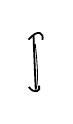
\begin{tikzpicture}[x=1em,y=1em]
\draw[line width=.65pt] (0,2.08) .. controls (.02,1.5) and (.06,.55) .. (.08,.15);
\draw[line width=.3pt] (.06,1.8) .. controls (.16,.9) and (.17,.35) .. (.08,.15);
\draw[line width=.65pt] (-.18,1.95) .. controls (.16,2.35) and (.38,2.2) .. (.32,1.94);
\draw[line width=.65pt] (-.17,.24) .. controls (.02,-.03) and (.28,.08) .. (.20,.29);
\end{tikzpicture}

\noindent\hspace*{1.6em}\begin{minipage}[t]{\dimexpr\linewidth-1.6em\relax}
$E$ est engendré par les \deleted{\unsure{objets|objet}} \unsure{sous-objet|sous-objets} de l'objet final\unsure{.} qui sont connexes, non vides et projectifs.
\end{minipage}

\noindent\hspace*{1.8em}
\begin{tikzpicture}[x=.08mm,y=-.08mm,baseline=(current bounding box.center)]\draw[line width=.5pt,line cap=round] (22,13)..controls(25,17)and(25,19)..(25,26) (25,30)..controls(26,49)and(23,80)..(26,96) (33,24)..controls(34,60)and(34,88)..(35,120);\draw[line width=1pt,line cap=round,line join=round] (24,32)--(34,20)--(37,27) (27,100)--(31,110) (24,112)..controls(27,120)and(30,120)..(35,123)--(35,108);\end{tikzpicture}

\noindent\hspace*{1.8em}\begin{minipage}[t]{\dimexpr\linewidth-1.8em\relax}
(\deleted{\unsure{où|Que}}\unsure{si|où|Ex.} $E=C^{\wedge}$) Tous les morphismes de $C$ sont des monomorphismes
\end{minipage}

\noindent\hspace*{.63\linewidth}\begin{tikzpicture}[x=1em,y=1em]
\draw[line width=.35pt] (0,.9)--(.27,.63);
\draw[line width=.5pt] (.04,.36)--(.17,.29);
\draw[line width=.5pt] (.22,.25)--(.56,0);
\draw[line width=.35pt] (.83,.37)--(.94,.25);
\draw[line width=.35pt] (1.00,.18)--(1.12,.02);
\end{tikzpicture}

\noindent\hspace*{2em}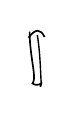
\begin{tikzpicture}[x=1em,y=1em]
\draw[line width=.6pt] (0,1.97) .. controls (.00,1.25) and (.18,.55) .. (.16,.27) .. controls (.16,.18) and (.12,.13) .. (.11,.10);
\draw[line width=.5pt] (.28,1.84) .. controls (.39,1.13) and (.39,.52) .. (.42,.10);
\draw[line width=.6pt] (-.04,1.75) .. controls (.21,2.08) and (.40,2.08) .. (.54,1.77);
\draw[line width=.6pt] (.08,.11) .. controls (.19,.02) and (.31,.03) .. (.42,.09)--(.39,-.03);
\end{tikzpicture}

\noindent\hspace*{2em}\begin{minipage}[t]{\dimexpr\linewidth-2em\relax}
(si $E=\operatorname{Top}(X)$, $X$ sobre) Pour $\forall\ x\in X$, l'ens des générisations de $x$ est\rlap{\hspace{.5em}\raisebox{-1em}{\begin{tikzpicture}[x=1em,y=1em]\draw[line width=.5pt] (0,0)--(.45,.11);\end{tikzpicture}}} un voisinage de $x$.
\end{minipage}

\noindent\hspace*{.74\linewidth}
\begin{tikzpicture}[x=1em,y=1em]
\draw[line width=.6pt] (.42,1.05)--(.54,.97);
\draw[line width=.65pt] (0,.70)--(.78,.23);
\draw[line width=.65pt] (.61,.53)--(.85,.35);
\draw[line width=.7pt] (.85,.67)--(1.00,.62);
\draw[line width=.6pt] (.48,.23)--(.66,.06);
\draw[line width=.5pt] (.89,.20)--(.95,.18);
\end{tikzpicture}\hspace{.8em}
\begin{tikzpicture}[x=.12mm,y=-.12mm,baseline=(current bounding box.center)]\draw[line width=.8pt,line cap=round,line join=round] (25,23)..controls(29,26)and(33,27)..(35,24)..controls(38,27)and(43,27)..(48,27);\draw[line width=.5pt,line cap=round] (34,39)--(53,45);\end{tikzpicture}

\vspace*{3em}
\noindent\hspace*{.94\linewidth}\begin{tikzpicture}[x=1em,y=1em]
\draw[line width=.65pt] (0,0)--(.26,.07);
\end{tikzpicture}
% archive sheet number: 48

\scanpage{50}
\mspage{\handwritten{6}}

\begingroup
\setbox0=\vbox{%
  \small
  \hsize=\linewidth
  \parindent=0pt
  \parskip=.45\baselineskip
  Pour la première assertion, on se ramène encore, par descente et en utilisant \deleted{1}\handwritten{4}.\handwritten{3}, au cas où $k$ est séparablement clos. Procédant comme dans la démonstration de \deleted{1}\handwritten{4}.6 , on déduit de \deleted{1}\handwritten{4}.5 et de l'hypothèse sur $L$ que $\underline{L}$ \deleted{provient} est isomorphe à l'image inverse d'un Module birigidifié $\underline{M}$ sur $A\mathbin{\mathrm{x}}Q$, et pour la première assertion de \deleted{1}\handwritten{4}.7, on est donc ramené au cas $A=P$. Or $\underline L$ définit un morphisme de schémas ponctués
  \[
    f\colon Q\handwritten{\longrightarrow}\underline{\mathrm{P}\deleted{\unsure{j|i}}\mathrm{ic}}_{P/k}\ ,
  \]
  qui se factorise nécessairement par le schéma abélien dual $P'$ de $P$. Soit $\underline{L}'$ l'image inverse du faisceau de Weil sur $P\mathbin{\mathrm{x}}P'$ par \deleted{$\mathrm{id}_{P}\mathbin{\mathrm{x}}\mathrm{id}$}
  \[
    \deleted{p}\mathrm{id}_{P}\mathbin{\mathrm{x}}f\colon P\mathbin{\mathrm{x}}Q\handwritten{\longrightarrow}P\mathbin{\mathrm{x}}P'\ ,
  \]
  c'est un Module birigidifié qui, par définition de $f$, ne diffère \deleted{q}de $\underline L$ que modulo l'image inverse d'un Module inversible $\underline M$ sur $P$. Comme $\underline L'$ et $\underline L$ ont une restriction triviale à $\deleted{\unsure{e|E}}P\mathbin{\mathrm{x}}e_{Q}$ , on en conclut que $\underline M$ est triv\unsure{\deleted{a}i\deleted{i}a|\deleted{i}a\deleted{a}i}l, donc que $\underline L$ est isomorphe à $\underline L'$. Or nous avons signalé dans VII 2.9.4 \deleted{p}que sur un produit de deux schémas abéliens, les correspondances divisorielles provenaient de biextensions. Il en résulte que $\underline L'$ , \deleted{\unsure{et en|et ea}} ou \unsure{\deleted{p}c|p}e qui revient au même, $\underline L$ , provient d'une biextension.\par

  Revenant au cas généfal ($P$ extension de $A$ par $L$), \unsure{\deleted{e}i\deleted{t}l|\deleted{i}e\deleted{l}t} reste à prouver que (\deleted{1}\handwritten{4}.7.1) est bien un isomorphisme. Mais cela résulte de la suite exacte des $\mathrm{B}\rlap{\begin{tikzpicture}[overlay,baseline=0pt,x=1em,y=1ex,line cap=round]
    \draw[line width=.5pt] (.02,-.35) -- (.23,-.35) -- (.27,-.7);
  \end{tikzpicture}}\bar{\mathrm{i}}\mathrm{ext}^{i}$ ($i=0,1$) associée à la suite exacte
  \[
    0\rlap{
\begin{tikzpicture}[overlay,baseline=0pt,x=1em,y=1ex,line cap=round]
      \draw[line width=.55pt] (.45,.35) .. controls (.12,-.1) and (.22,-.65) .. (.65,-1.4);
    \end{tikzpicture}}\handwritten{\longrightarrow}L\handwritten{\longrightarrow}P\handwritten{\longrightarrow}A\handwritten{\longrightarrow}0\ ,
  \]
  et des relations
  \[
    \operatorname{Biext}^{o}(L,Q;\underline G_{m})=0\ ,\quad
    \operatorname{Biext}^{1}(L\overset{\unsure{\mathrm{x}|\deleted{\mathrm{x}}}}{,}Q;\underline G_{m})=0\ ,
  \]
  dont la premièr\unsure{\deleted{u}e|ë} est un cas parti\unsure{\deleted{v}c|\deleted{c}v}ulier de l'assertion de rigidité faite dans \deleted{1}\handwritten{4}.\handwritten{3} , et la deuxième n'est autre que le premier cas de \deleted{1}\handwritten{4}.6.\par

  \setbox2=\vbox{%
    \hsize=\linewidth
    \parindent=0pt
    \uline{Corollaire} \deleted{1}\handwritten{4}.8. Sous les conditions de \deleted{1}\handwritten{4}.7, supposons que $Q$ soit extension d'un groupe algébrique $B$ (néces\unsure{\inserted{s}a|\deleted{s}a}irement lisse et connexe) par un\par
  }%
  \edef\corollaryheight{\the\ht2}
  \noindent\hbox{%
    \rlap{\begin{tikzpicture}[overlay,baseline=0pt,x=1em,y=\corollaryheight,line cap=round]
      \draw[line width=.65pt] (-.75,1) .. controls (-.84,.93) and (-.81,.6) .. (-.8,.4)
        .. controls (-.78,.2) and (-.72,.08) .. (-.7,0);
      \draw[line width=1.05pt] (-.77,.25) -- (-.7,0);
    \end{tikzpicture}}%
    \box2
  }\par
}%
\edef\scanblockwidth{\the\wd0}
\edef\scanblockheight{\the\ht0}
\noindent\hbox{%
  \rlap{\raise\ht0\hbox{%
    \begin{tikzpicture}[overlay,baseline=0pt,x=\scanblockwidth,y=-\scanblockheight,line cap=round]
      \draw[black!55,line width=.5pt]
        (.125,-.015) .. controls (.12,-.04) and (.15,-.03) .. (.17,.01)
        .. controls (.27,.17) and (.60,.65) .. (.746,.98);
      \draw[black!28,line width=.45pt]
        (.516,.018) .. controls (.56,.095) and (.73,.37) .. (.849,.564);
      \draw[black!45,line width=.5pt]
        (.059,.516) .. controls (.10,.523) and (.12,.55) .. (.136,.59)
        .. controls (.22,.74) and (.31,.86) .. (.372,.917);
    \end{tikzpicture}%
  }}%
  \box0
}\par
\endgroup

% archive sheet number: 49

\scanpage{51}
\hfill SGA 5
% archive sheet number: 50

\scanpage{57}
\noindent\begin{minipage}{.60\linewidth}
\centering
INSTITUT\\
DES HAUTES ÉTUDES SCIENTIFIQUES\\[-.4ex]
\rule{1.4cm}{.4pt}
\end{minipage}

\bigskip
\noindent\begin{minipage}[t]{.31\linewidth}
\raggedleft
SGA 6 \uline{$\overline{\mathrm{V}\deleted{\unsure{\mathrm{I}|\mathrm{II}}}}$}
\end{minipage}\hfill
\begin{minipage}[t]{.64\linewidth}
Donner interprétation de
la relation entre ``\unsure{suites|suite}
mult. de polynômes'' de
Hirzebruch, et séries formelles,
par la 'opération $f*g$ \ldots
\end{minipage}

\medskip
\noindent\rule{\linewidth}{.4pt}

\medskip
\noindent\hspace*{.08\linewidth}Introduction, page de garde

\medskip
\noindent\hspace*{.18\linewidth}Mentionner Serre et Jouanolou\\[1ex]
\hspace*{.28\linewidth}sur page de garde ?
% archive sheet number: 56
